\chapter{Implementación}
\label{cap:implementacion}

En éste capítulo introduciremos los detalles más relevantes del desarrollo realizado para este trabajo. Comenzaremos mostrando la integración de nuestro sistema de NLG con \textit{Fastest}, viendo el modo de uso y los nuevos comandos introducidos para la generación de descripciones en lenguaje natural. Luego presentaremos los aspectos más destacados de nuestra implementación presentes en cada una de las etapas del \emph{pipeline}.

\section{Integración con \emph{Fastest}}

La implementación realizada para este trabajo se encuentra incluida en la última versión de \emph{Fastest}, cuyo código está disponible públicamente\footnote{\url{http://github.com/rosacris/fastest}}. La mayor parte del código referente a este trabajo la podremos encontrar dentro del paquete \textit{nlg}.

\subsection*{Requisitos}

%TODO referenciar tutorial / notas a algun sitio más lindo
Para garantizar el correcto funcionamiento de Fastest y nuestro sistema de NLG, deberemos cumplir con los siguientes requerimientos:

\begin{itemize}
 \item  \emph{Fastest 1.6 o superior}: la distribución de éste incluye un pequeño manual de uso.
 \item  \emph{Java SE Runtime Environment 1.6 o superior}: requerido para el correcto funcionamiento de \emph{Fastest}.
 \item  \emph{SWI\_Prolog\footnote{\url{http://www.swi\_prolog.org/}}}: también requerido para el correcto funcionamiento de Fastest.
 \item  \emph{FreeLing 3.1\footnote{\url{http://nlp.lsi.upc.edu/freeling/}. Hemos creado un pequeño tutorial para instalación de \emph{FreeLing} en \emph{Ubuntu}; disponible en \url{http://gist.github.com/juliandt/}}.}: suite de análisis de lenguajes, necesaria para el módulo de NLG de \emph{Fastest}
\end{itemize}

\subsection{Modo de uso}

Como resultado de este trabajo introdujimos un nuevo comando en \textit{Fastest}, el comando \texttt{showdesc}. Podremos usar el mismo para generar la descripción de una o más clases de prueba, pasándole el título deseado para el documento junto con el o los nombres de las clases de prueba a traducir. También es posible pasar como argumento el nombre de una operación de la especificación y nuestro sistema buscará todas las clases de prueba generadas para esa operación produciendo luego las descripciones para las mismas. En la figura, \ref{ej:showdesc_fastest} podemos ver la ayuda de \textit{Fastest} para el comando anterior.

\begin{figure}[H]
\centering
\begin{Verbatim}[frame=single,fontsize=\scriptsize]
showdesc [-t <title>] [<sch_name>]
	Generates natural language description for specified schemas.
\end{Verbatim}
\caption{Ayuda para el comando showdesc en \emph{Fastest}}
\label{ej:showdesc_fastest}
\end{figure}

Veremos a continuación un ejemplo de uso del comando \texttt{showdesc}, mediante un ejemplo similar al introducido en la sección \ref{sec:fastest} (donde ilustramos el funcionamiento general de \textit{Fastest}):

\begin{figure}[H]
\centering
\begin{Verbatim}[frame=single,fontsize=\scriptsize]
Fastest version 1.6, (C) 2013, Maximiliano Cristiá
Loading pruning rewrite rules...
Loading pruning theorems...
Fastest> loadspec symbolTable.tex
Loading specification..
Specification loaded.
Fastest> selop LookUp
Fastest> addtactic LookUp SP \in s? \in \dom st      
Fastest> genalltt
Generating test tree for 'LookUp' operation.
Fastest> showdesc -t "Descripción clase de prueba: LookUp_SP_1" LookUp_SP_1 

\documentclass{article}
\title{Descripción clase de prueba: LookUp_SP_1}

\begin{document}
\maketitle

LookUp_SP_1: Se intenta buscar un simbolo en la tabla
Cuando:
\begin{itemize}
 \item{El simbolo a buscar pertenece a los simbolos cargados en la tabla.}
 \item{El simbolo a buscar es el único elemento en los simbolos cargados en la tabla.}
\end{itemize}

\end{document}
\end{Verbatim}
\caption{Comandos para generación de descripciones en \emph{Fastest}}
\label{ej:comandos_fastest_nlg}
\end{figure}


Por otro lado, para poder hacer uso de las designaciones presentes en la especificación hemos definido un nuevo entorno y un nuevo comando para facilitarnos el parseo de las mismas. En la figura \ref{img:comandos_designaciones} podemos observar el código necesario que el especificador deberá incluir junto a la especificación.

\begin{figure}[H]
\centering
\begin{Verbatim}[frame=single,fontsize=\scriptsize]
\newenvironment{designations}[1]
  {\begin{leftbar}
    \begin{list}{}{\setlength{\labelsep}{0cm}
                   \setlength{\labelwidth}{0cm}
                   \setlength{\listparindent}{0cm}
                   \setlength{\rightmargin}{\leftmargin}}}
  {\end{list}\end{leftbar}}

\newcommand{\desig}[2]{\item #1 $\approx #2$}
\end{Verbatim}
\caption{Comandos necesarios para la definición de designaciones en la especificación}
\label{img:comandos_designaciones}
\end{figure}

Luego deberá introducir las designaciones haciendo uso del nuevo comando definido. En la figura \ref{ej:comandos_designaciones} podemos ver un bloque de designaciones haciendo uso del comando presentado en la figura \ref{img:comandos_designaciones}. Podemos observar que es posible pasarle un nombre de esquema como parámetro al entorno \texttt{designations} para delimitar el \textit{scope} de las variables designadas. De no pasarle un nombre de esquema como parámetro el sistema considerará que el scope del bloque de designaciones es toda la especificación (utilizamos esta alternativa por ejemplo para designar nombres de esquemas, tipos básicos, etc.).

\begin{figure}[H]
\centering
\begin{Verbatim}[frame=single,fontsize=\scriptsize]
\begin{designations}{}
  \desig{se intenta buscar un simbolo en la tabla}{LookUp}
  \desig{se intenta actualizar la tabla de simbolos}{Update}
\end{designations}

\begin{designations}{LookUp}
  \desig{el simbolo a buscar}{s?}
  \desig{la tabla de simbolos}{st}
  \desig{simbolos cargados en la tabla}{\dom st}
\end{designations}
\end{Verbatim}
\caption{Ejemplo designaciones \textit{SymbolTable}}
\label{ej:comandos_designaciones}
\end{figure}

\section{Detalles de la implementación}

En esta sección detallaremos los aspectos más importantes de la implementación realizada. Para la misma respetamos la arquitectura y desarrollo realizado a lo largo de este trabajo. Sin embargo podremos observar algunas diferencias menores, como por ejemplo, la necesidad de modificar los nombres de las entidades intermedias utilizadas entre las distintas etapas del \textit{pipeline} para respetar las convenciones de estilo utilizadas en Fastest.

A continuación describiremos la función de los componentes más importantes usados en cada etapa de nuestro sistema.

\subsection{\textit{Document Planner}}

El módulo \emph{DocumentPlanner} será el encargado de llevar a cabo las tareas de determinación de contenido y estructuración del documento detalladas en el capítulo \ref{cap:document_planning}. En la figura \ref{fig:imp_documentplanner} podemos observar los componentes más importantes involucrados en esta etapa, cuya función describiremos a continuación. 

\begin{figure}[H]
  	\centering
	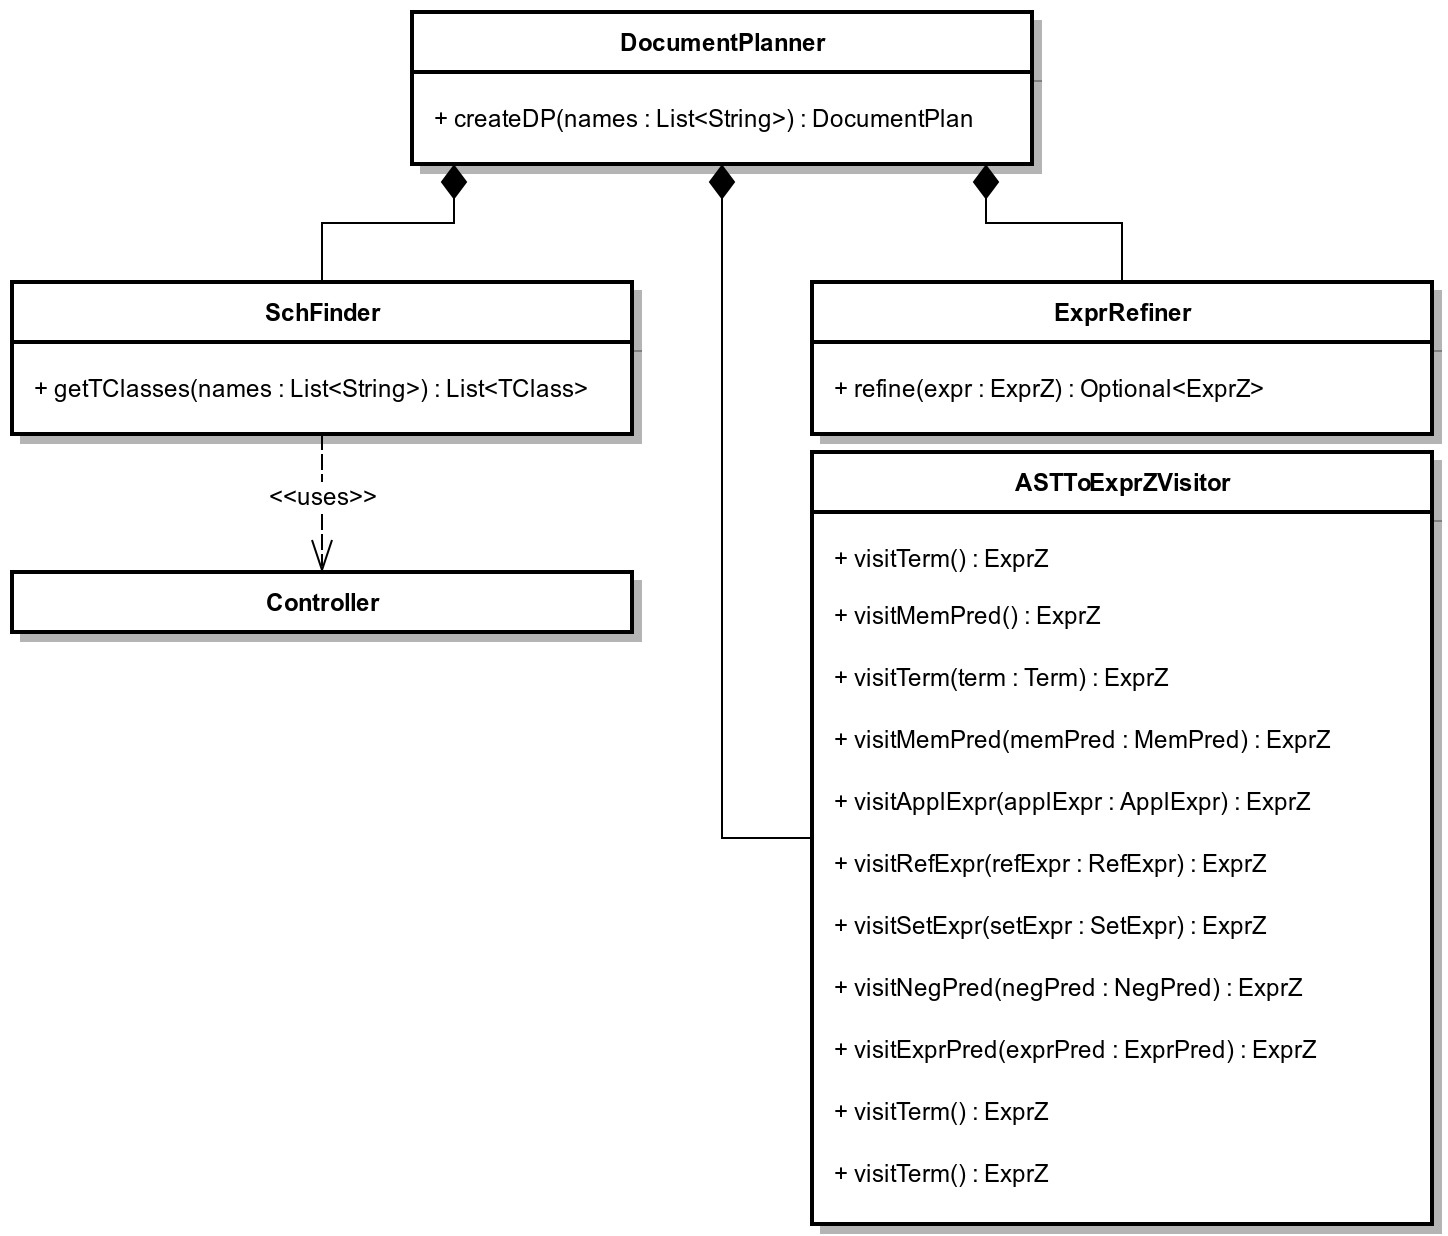
\includegraphics[scale=0.25]{img/documentplanner_imp.png}
	\caption{Diagrama clases para \textit{DocumentPlanner}}
  	\label{fig:imp_documentplanner}
\end{figure}

\bigskip
\noindent
\textbf{DocumentPlanner.} Es el módulo encargado de crear un \textit{document plan} a partir de la entrada de nuestro sistema. Construye los mensajes y estructuras intermedias de éste, delegando las tareas de determinación de contenido en los módulos que describiremos a continuación.

\bigskip
\noindent
\textbf{SchFinder.} La tarea de selección detallada en la sección \ref{cap:determinacion_contenido} será desarrollada por este módulo, que será el encargado de recuperar el conjunto de clases de prueba indicadas. El mismo posee una referencia al módulo \textit{Controller}\footnote{\textit{Controller} es el módulo encargado de mantener las referencias a elementos de la especificación, arboles de prueba, etc.} de Fastest que le permitirá identificar y recuperar las clases de prueba necesarias. 


\bigskip
\noindent
\textbf{ExprRefiner.} Es la \textit{fachada} \cite{gof} encargada de delegar los distintos procesamientos a realizar sobre las expresiones a fin de desarrollar las tareas de eliminación de tautologías y reducción de expresiones estudiadas en la sección \ref{cap:determinacion_contenido}. Podemos observar que utilizamos la clase \texttt{Optional} de Java 8 para modelar el hecho de que el método \texttt{refine()} podría no devolver un valor, por ejemplo en el caso que la expresión procesada sea una tautología y no deba ser incluida en el \textit{document plan}. En el capítulo \ref{cap:conclusion} propondremos como trabajo a realizar, la implementación de nuevas tareas de razonamiento con los datos; será en esta clase en la que deberemos agregar las el comportamiento necesario para contemplar dichas tareas (cada una de éstas debería estar encapsulada un un módulo separado y el módulo ExprRefiner debería tener una referencia a los mismos e implementar las llamadas a los métodos de correspondientes).

\bigskip
Fastest utiliza el \textit{framework} CZT\footnote{\url{http://czt.sourceforge.net/}} que integra un conjunto de herramientas para trabajar con el lenguaje de especificación Z. La forma en la que CZT modela las expresiones de Z nos resultó compleja para este trabajo, por lo que decidimos transformar las expresiones contempladas dentro del alcance de este trabajo a un modelo más simple (lo que simplificó la implementación del algoritmo de lexicalización, por ejemplo). En la figura \ref{fig:imp_exprz} podemos observar la jerarquía de clases de las expresiones utilizadas en este trabajo para modelar las expresiones Z. 

\begin{figure}[H]
  	\centering
	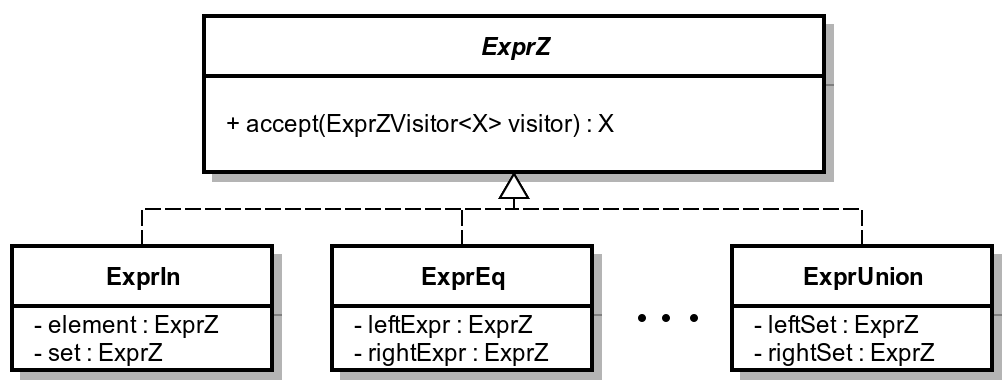
\includegraphics[scale=0.31]{img/exprz_imp.png}
	\caption{Diagrama jerarquía de clases para ExprZ}
  	\label{fig:imp_exprz}
\end{figure}

\bigskip
\noindent
\textbf{ASTToExprZVisitor.} Este módulo será el responsable de la transformación entre el modelo de CZT y el utilizado por este trabajo presentado en la figura \ref{fig:imp_exprz}.


\subsection{\textit{Microplanner}}

En esta sección presentaremos los componentes encargados de la tarea de \textit{microplanning} detallada en el capítulo \ref{cap:microplanning}. En la figura \ref{fig:imp_microplanner} podemos observar los módulos involucrados en la implementación de esta tarea.

\begin{figure}[H]
  	\centering
	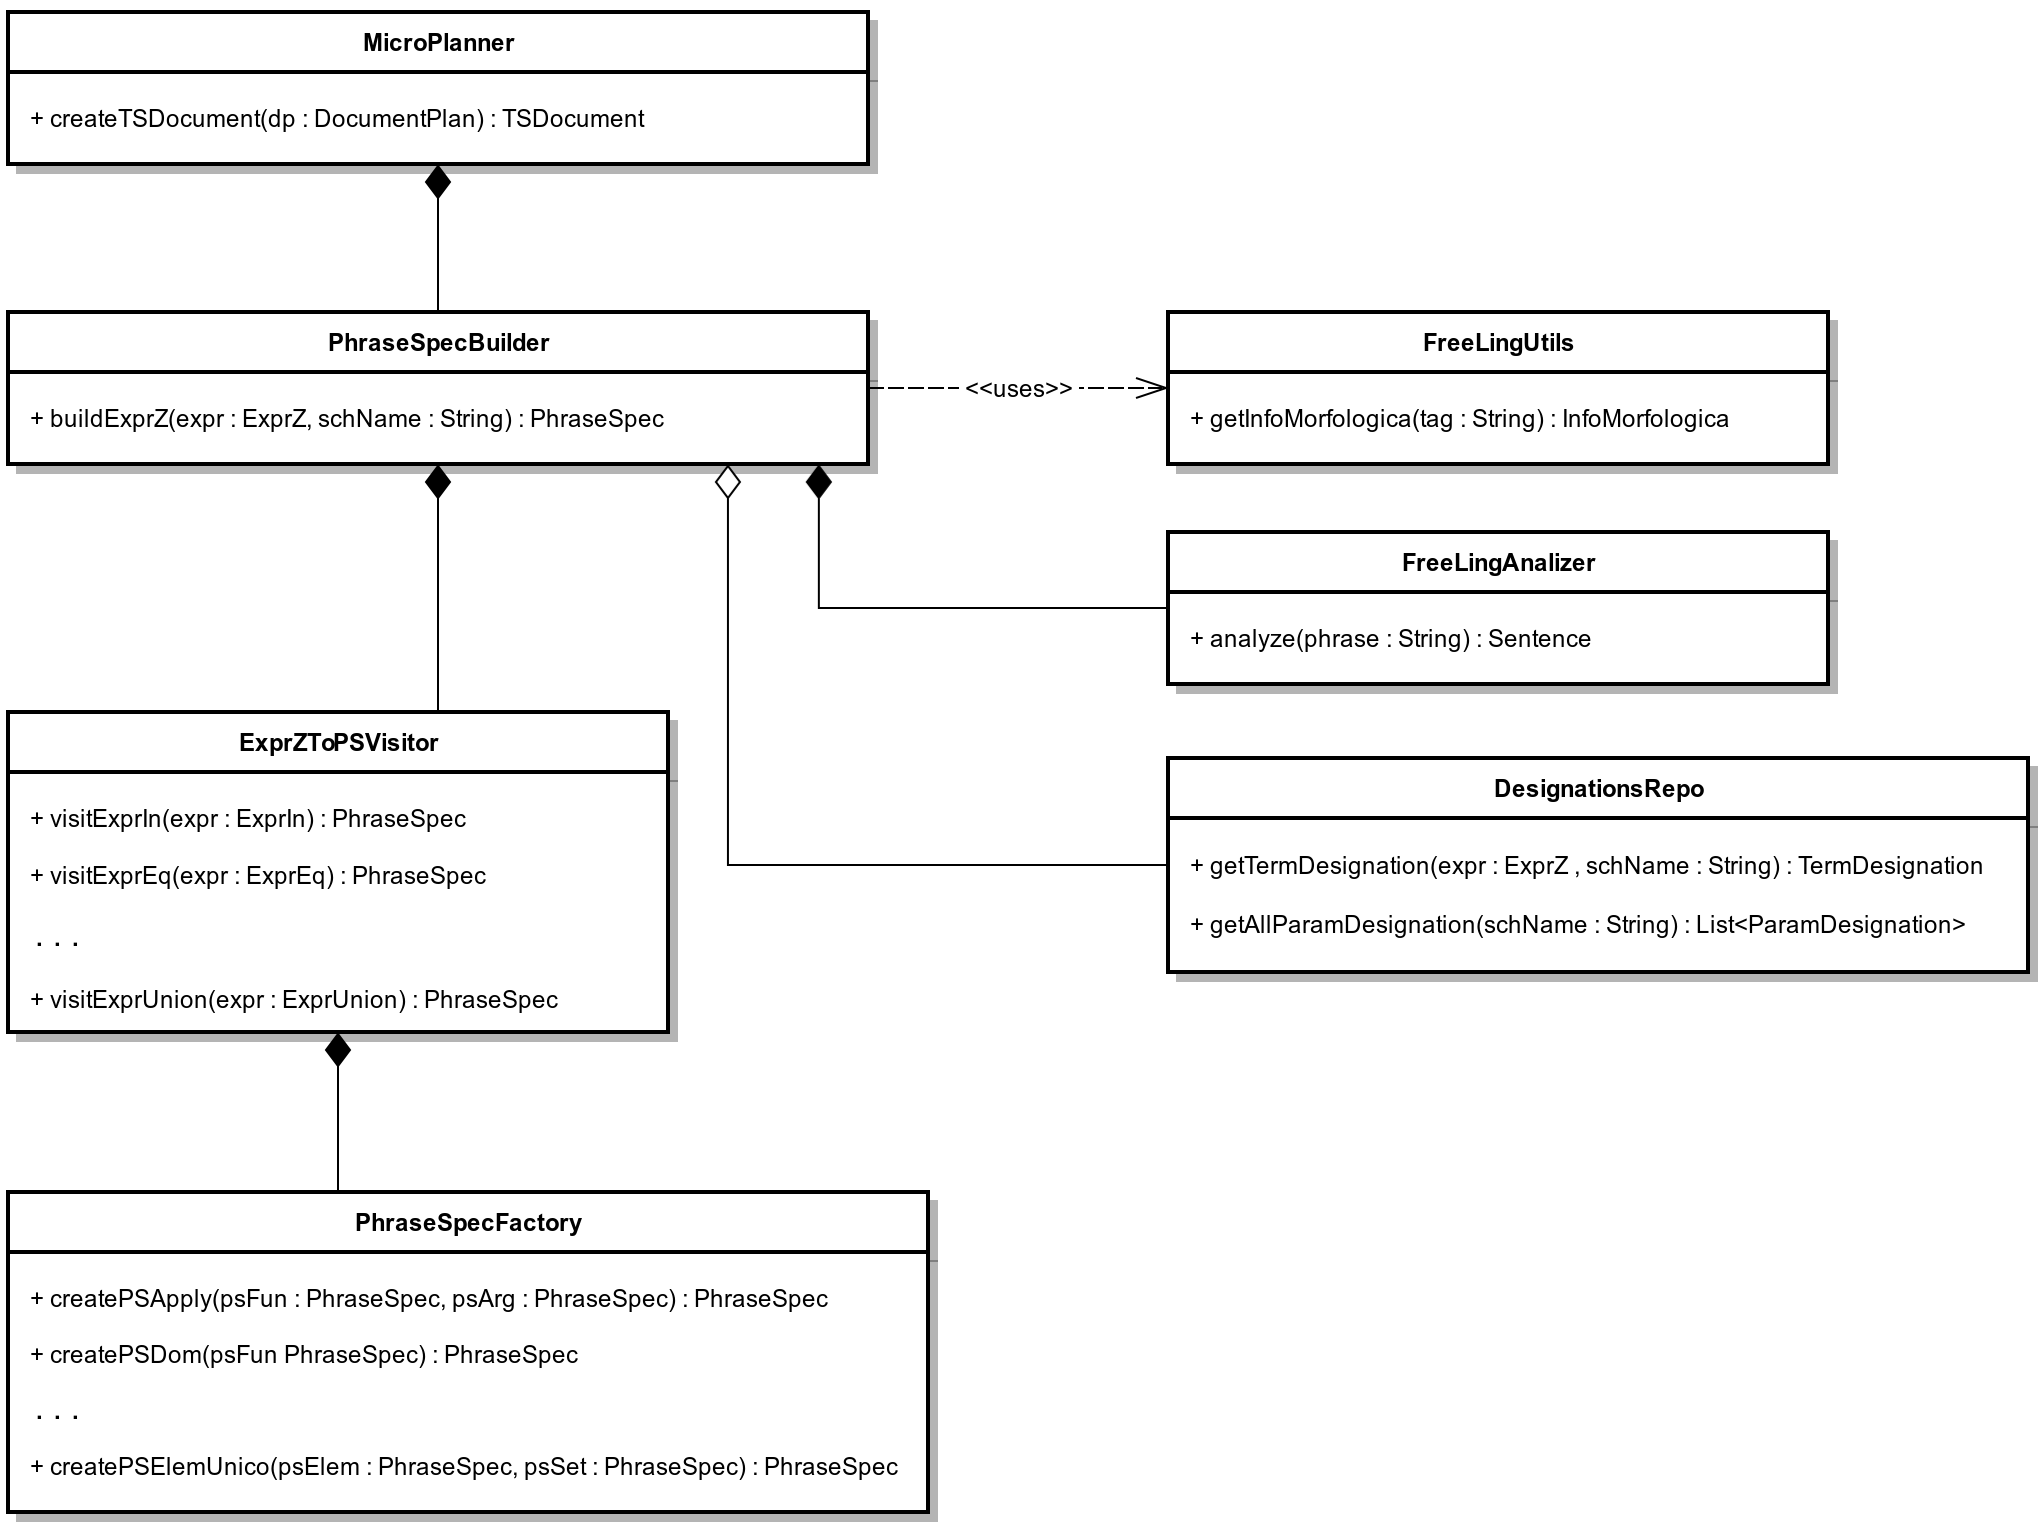
\includegraphics[scale=0.2]{img/microplanner_imp.png}
	\caption{Diagrama clases para \textit{Microplanner}}
  	\label{fig:imp_microplanner}
\end{figure}

\bigskip
\noindent
\textbf{MicroPlanner.} Es el módulo principal de esta etapa, encargado de construir la especificación del documento a partir del \textit{document plan} generado por la etapa anterior. Éste delega la tarea de lexicalización en el módulo \textit{PhraseSpecBuilder} que presentaremos a continuación.

\bigskip
\noindent
\textbf{PhraseBuilder.} Este módulo implementa la tarea de lexicalización detallada en el capítulo \ref{cap:microplanning}, la función del mismo será construir una especificación de frase a partir de una expresión Z. Para realizar esta tarea necesitaremos recorrer el modelo utilizado para las expresiones Z. Encapsulamos este trabajo en el módulo \textit{ExprZToPSVisitor}, encargado del análisis de casos para las distintas expresiones y sus posibles combinaciones de acuerdo a la definición presentada en la sección \ref{sec:microplanning_lexicalization}.

\bigskip
\noindent
\textbf{ExprZToPSVisitor.} Encapsula las reglas de lexicalización para todas las posibles expresiones y combinaciones de las mismas. Implementa la función auxiliar \textsc{lexicalización'()} utilizada en el bosquejo de la figura \ref{fig:algoritmo_lexicalizacion}. Utilizamos el patrón de diseño \textit{visitor} \cite{gof} para iterar sobre la estructura de las distintas expresiones Z modeladas por nuestro sistema.

\bigskip
\noindent
\textbf{PhraseSpecFactory.} Construir y componer las especificaciones de frase de nuestro sistema resulta una tarea relativamente compleja. Es por esto que encapsulamos esta funcionalidad en el módulo \textit{PhraseSpecFactory} encargado de construir apropiadamente las distintas especificaciones de frase de nuestro sistema. Por ejemplo: \texttt{createPSElemUnico()} tomará dos especificaciones de frase y las compondrá para generar una nueva especificación para la frase \textit{``... es el único elemento de ...''}, siendo las dos especificaciones mencionadas anteriormente las encargadas de modelar el texto que precede y antecede respectivamente a la anterior.

\bigskip
\noindent
\textbf{FreeLingAnalizer.} Utilizamos el analizador morfosintáctico \textit{FreeLing} para obtener las características morfológicas de los distintos constituyentes de las frases utilizadas en las designaciones. Este módulo tendrá la tarea de interactuar con las librerías provistas por la herramienta proveyéndonos de la información necesaria (como el núcleo de la frase, su género, número, etc.) para poder construir una especificación de frase a partir de una designación.

\bigskip
\noindent
\textbf{FreeLingUtils.} Contiene algunos métodos útiles para el trabajo con \textit{FreeLing}. Por ejemplo, \textit{FreeLing} genera una estructura en la que etiqueta cada palabra con anotaciones morfosintácticas. El método \texttt{getInfoMorfologica()} procesa estas anotaciones produciendo una estructura más sencilla con la que trabajará nuestro sistema.

\bigskip
\noindent
\textbf{DesignationsRepo.} Es necesario para el algoritmo de lexicalización saber si una expresión se encuentra designada y, en ese caso, necesitará saber cúal es su designación. Será a través de este módulo que podrá acceder a las designaciones presentes en la especificación. El mismo se inicializa al cargar la especificación en Fastest. 

%TODO cambiar nombres a español
\subsection{\textit{Surface Realizer}}

Finalmente, el módulo \emph{SurfaceRealizer} será el encargado de generar el texto de superficie para el documento final en base a una especificación del mismo. En esta etapa se realizan las tareas de realización estructural y lingüística presentadas en el capítulo \ref{cap:realization}. En la figura \ref{fig:imp_surfrealizer} podemos ver los componentes más relevantes involucrados en esta etapa, cuya función describiremos a continuación. 

\begin{figure}[H]
  	\centering
	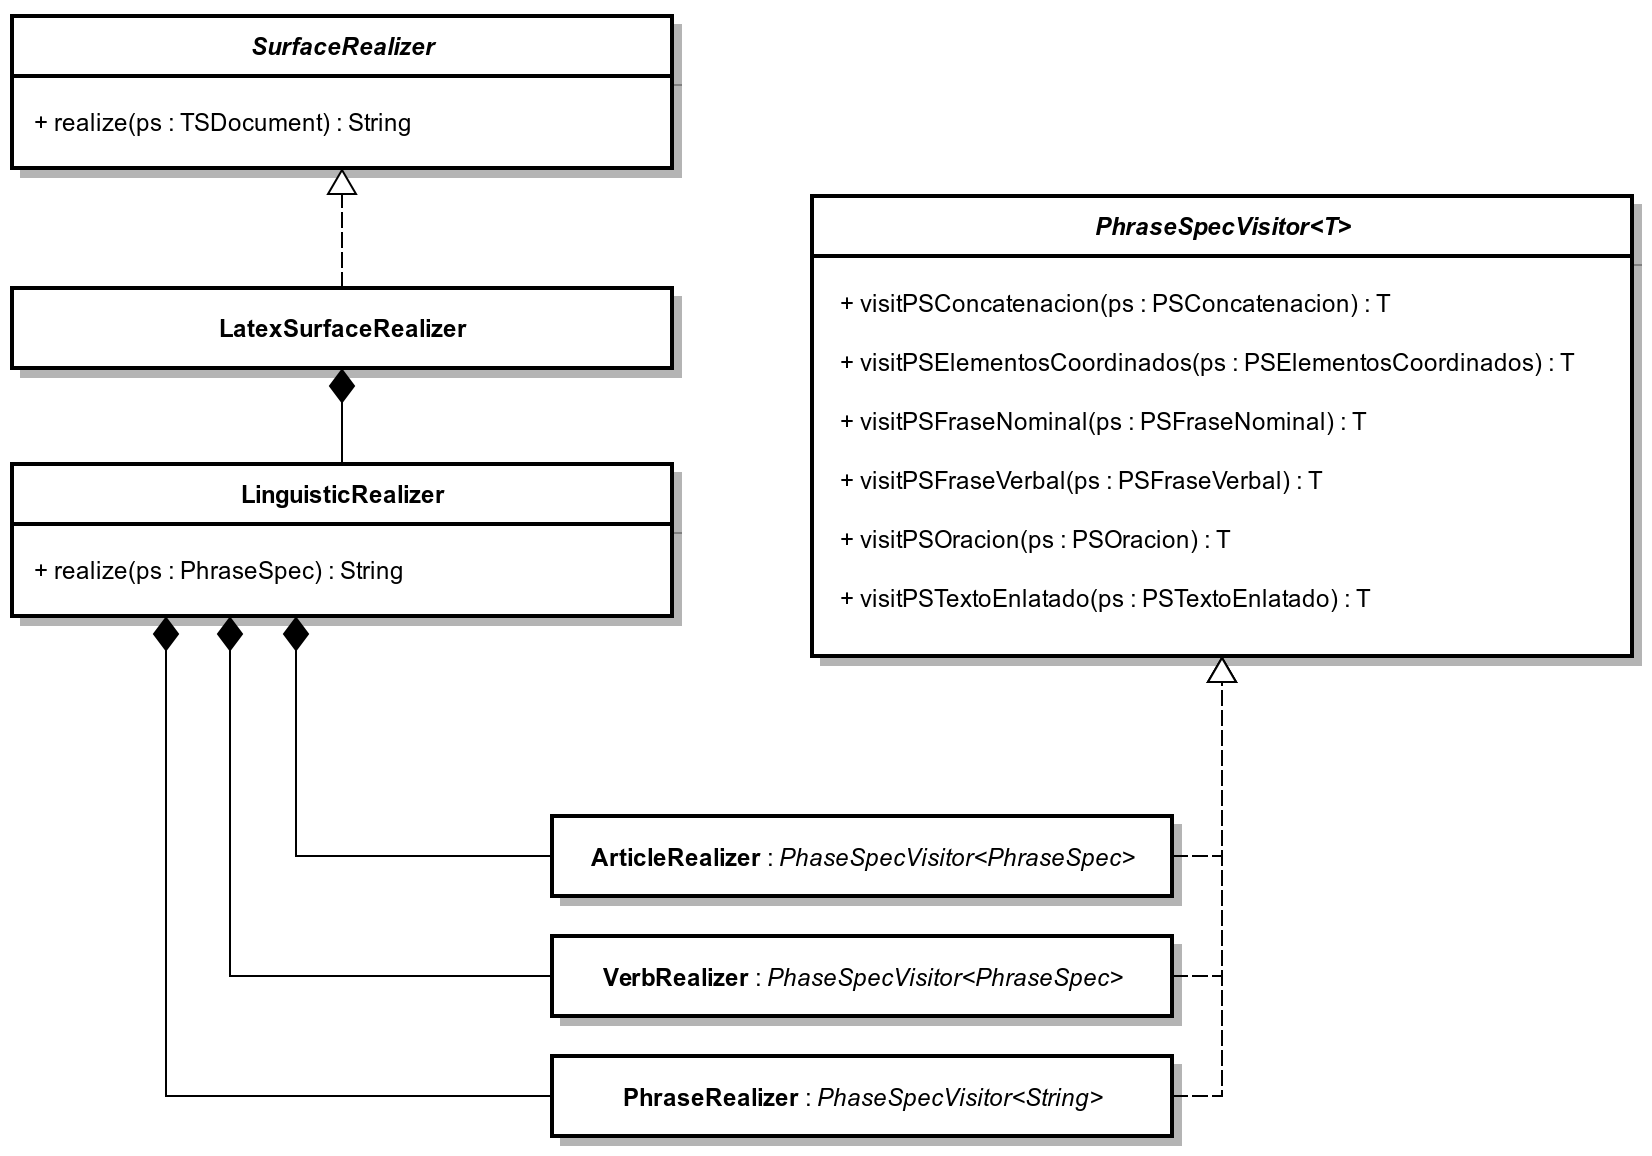
\includegraphics[scale=0.20]{img/realizer_imp.png}
	\caption{Diagrama clases para \textit{Surface Realizer}}
  	\label{fig:imp_surfrealizer}
\end{figure}

\bigskip
\noindent
\textbf{SurfaceRealizer.} Como mencionamos en la sección \ref{cap:realization} la tarea de realización estructural resulta dependiente del sistema de presentación utilizado. Es por esto que definimos la interfaz abstracta \textit{SurfaceRealizer} y una implementación especifica encargada de producir código \LaTeX~apropiado para el documento final. El método principal de esta clase toma una especificación del documento final y tiene la misión de producir el texto en lenguaje natural esperado, para esto deberá hacer uso del \textit{LinguisticRealizer} para lograr la realización lingüística de cada una de las especificaciones de frase presentes en la especificación de documento dada. 


\bigskip
\noindent
\textbf{LinguisticRealizer.} Es el módulo encargado de la realización lingüística. Es responsabilidad de este módulo asegurarse de que las frases del texto generado respeten las reglas gramaticales introducidas en el capítulo \ref{cap:linguistic_realization}. Éste hace uso de los módulos \textit{ArticleRealizer} y \textit{VerbRealizer} para resolver las cuestiones de concordancia gramatical, delegando la generación del texto final en el módulo \textit{PhraseRealizer}. 

\bigskip
\noindent
\textbf{PhraseSpecVisitor.} Utilizamos el patrón \textit{visitor} para iterar sobre la estructura de las especificaciones de frase. A continuación veremos la función de las tres implementaciones más importantes de esta interfaz. 

\bigskip
\noindent
\textbf{ArticleRealizer.} Es el módulo encargado de recorrer la estructura de una especificación de frase y escoger el articulo apropiado (de ser necesario en una frase nominal) de forma tal que concuerde según las reglas gramaticales introducidas previamente. El artículo será agregado sobre la misma estructura utilizada para la especificación de frase.

\bigskip
\noindent
\textbf{VerbRealizer.} Este módulo tiene la responsabilidad de conjugar el verbo de una oración (establecido en infinitivo por el \textit{microplanner}) y escoger el atributo apropiado en caso de ser un verbo copulativo, teniendo en cuenta los aspectos gramaticales detallados en la sección \ref{cap:linguistic_realization}. Al igual que con \textit{ArticleRealizer}, reutilizaremos la estructura utilizada para la especificación de frases para establecer el verbo correcto y atributo (reemplazando el verbo infinitivo por el verbo correctamente conjugado y el atributo previamente establecido por el atributo correspondiente).

\bigskip
\noindent
\textbf{PhraseRealizer.} Será el módulo finalmente encargado de recorrer la estructura de una especificación de frase y generar el texto final correspondiente a la misma. En esta etapa casi todo el trabajo fue realizado. La función de este módulo será extraer el texto contenido en la especificación de frase con el fin de generar la frase final respetando el orden establecido e introduciendo los espacios y signos de puntuación necesarios. Es importante aclarar que resulta necesario que ejecutemos en primer instancia las tareas realizadas por \textit{PhraseSpecVisitor} y \textit{VerbRealizer} ya que \textit{PhraseRealizer} asumirá que ya fueron resueltos previamente todos los aspectos gramaticales.

\section{Resumen del capítulo}
En este capítulo presentamos el prototipo desarrollado como resultado de este trabajo. Mostramos su integración con Fastest, presentando los nuevos comandos introducidos para la generación de descripciones de clases de prueba y describimos su modo de uso. Detallamos también la forma en la que el especificador debe escribir las designaciones para que el sistema pueda hacer uso de ellas. Finalmente comentamos los aspectos más interesantes de la implementación realizada junto con algunas recomendaciones para futuras modificaciones.